\documentclass{article}
\usepackage[a4paper, landscape, left=1cm, right=1cm, top=1.7cm, bottom=1.2cm]{geometry}
\usepackage[utf8]{inputenc}
\usepackage[english]{babel}

\usepackage{multicol}
\usepackage{amssymb}
\usepackage{amsmath}
\usepackage{mathtools}
\usepackage{cancel}

\usepackage{graphicx}

\usepackage{enumitem}
% declare delimiter for ceil and floor from mathtools
\DeclarePairedDelimiter\ceil{\lceil}{\rceil}
\DeclarePairedDelimiter\floor{\lfloor}{\rfloor}

% remove indentaion
\setlength\parindent{0pt}

\usepackage{fancyhdr} % to change header and footers

\pagestyle{fancy} % Turn on the style
\fancyhf{} % Start with clearing everything in the header and footer
% Set the right side of the footer to be the page number
\fancyfoot[R]{\thepage}

% Redefine plain style, which is used for titlepage and chapter beginnings
% From https://tex.stackexchange.com/a/30230/828
\fancypagestyle{plain}{%
    \renewcommand{\headrulewidth}{0pt}%
    \fancyhf{}%
    \fancyfoot[R]{\thepage}%
}
\rhead{Austin Santoso}
\lhead{CS3230 Cheatsheet}
\rfoot{Page \thepage}

\setlength{\columnseprule}{0.1pt}


\begin{document}
\begin{multicols*}{4}

\section{Week 1-Reasoning and asymptotic analysis}
\subsection{Correctness of algorithm}

\subsubsection{Correctness of iterative algorithm}
A \textbf{loop invariant} is:
\begin{itemize}
\item true at the beginning of an iteration
\item remains true at the beginning of the next iteration
\end{itemize}

To proof the correctness of an iterative algorithm, We need to show 3 things:

\begin{itemize}
\item \textbf{Initialization:} The invariant is true before the first iteration of the loop.
\item \textbf{Maintenance:} If the invariant is true before an iteration, it remains true before the next iteration.
\item \textbf{Termination:} When the algorithm terminates, the invariant provides a useful property for showing correctness.
\end{itemize}

\subsubsection{Correctness of recursive algorithm}

To proof the correctness of an iterative algorithm:
\begin{itemize}
\item Use strong induction
\item Prove base cases
\item Show algorithm works correctly assuming algorithm works correctly for smaller cases.
\end{itemize}

\subsection{Efficiency}
\textbf{Asymptotic Analysis} is a method of describing the limiting behavior.
Asymptotic notations:
\begin{itemize}
\item $O$-notation (BIG-O)\\(upper bound)
	\begin{itemize}
	\item $O(g(n))=\{f(n):$ there exist constants $c > 0$, $n_0 > 0$ such that $0 \leq f(n) \leq cg(n)$ for all $n \geq n_0\}$
	\end{itemize}
	
\item $\Theta$-notation (Theta)\\(tight bound)
	\begin{itemize}
	\item $\Theta (g(n))=\{f(n):$ there exist constants $c_1 > 0$, $c_2 > 0$, $n_0 > 0$ such that $0 \leq c_1 g(n) \leq f(n) \leq c_2 g(n)$ for all $n \geq n_0\}$
	\end{itemize}
	
\item $\Omega$-notation (BIG-Omega)\\(lower bound)
	\begin{itemize}
	\item $\Omega (g(n))=\{f(n):$ there exist constants $c > 0$, $n_0 > 0$ such that $0 \leq cg(n) \leq f(n)$ for all $n \geq n_0\}$
	\end{itemize}

\item $o$-notation (small-o)\\(tight upper bound)
	\begin{itemize}
	\item $o(g(n))=\{f(n):$ for any constant $c > 0$, there is a constant $n_0 > 0$ such that $0 \leq f(n) < cg(n)$ for all $n \geq n_0\}$
	\end{itemize}
	
\item $\omega$-notation (small-omega)\\(lower bound)
	\begin{itemize}
	\item $\omega (g(n))=\{f(n):$ for any constant $c > 0$, there is a constant $n_0 > 0$ such that $0 \leq cg(n) < f(n)$ for all $n \geq n_0\}$
	\end{itemize}
\end{itemize}


\section{Week 2-Recurrence and Mater Theorem}

\subsection{Properties of\\functions (MATHS)}
\subsubsection{Exponential}
\begin{displaymath}
a^{-1} = 1/a
\end{displaymath}
\begin{displaymath}
(a^m)^n = a^{mn}
\end{displaymath}
\begin{displaymath}
a^m a^n = a^{m+n}
\end{displaymath}
\begin{displaymath}
e^x \geq 1+x
\end{displaymath}
\subsubsection{Logarithm}
\[
\lg n = \
\
\log_2 n
\]
\[
\ln n = \log_e n
\]
\[
\lg^k n = (\lg n)^k
\]
\[
lg\, lg\, n = lg(lg\, n))
\]
\[
a = b^{\log_b a}
\]
\[
\log_c (ab) = \log_c a + \log_c b
\]
\[
\log_b a^n = n \log_ba
\]
\[
\log_b a = \frac{\log_c a}{\log_c b}
\]
\[
\log_b (1/a) = - \log_b a
\]
\[
\log_b a = \frac{1}{\log_a b}
\]
\[
a^{\log_b c} = c^{\log_b a}
\]
Stirling's approximation
\[
n! = \sqrt{2 \pi n} \left( \frac{n}{e} \right) ^n \left( 1+ \theta \left( \frac{1}{n} \right) \right)
\]
\[
\log(n!) = \theta (n\, \lg n)
\]

\subsubsection{Summation}
Arithmetic Series
\begin{align*}
\sum_{k=1}^{n}k&=1+2+3+...n\\
&=\frac{1}{1}n(n+1)=\Theta(n^2)
\end{align*}

\noindent Geometric Series
\begin{align*}
\sum_{k=1}^{n}x^k= 1 + x^2 + x^3 + ... x^n\\
=\frac{x^{n+1}-1}{x-1}\\
\sum_{k=1}^{\infty}x^k=\frac{1}{1-x} \text{when} \mid x \mid <1
\end{align*}

\noindent Harmonic Series
\begin{align*}
H_n =& 1 + \frac{1}{2} + \frac{1}{3} + ... + \frac{1}{n}\\
=&\sum_{k=1}^{n}\frac{1}{k}\\
=&\ln n + O(1)
\end{align*}


\noindent Telescoping Series
\begin{align*}
\text{For any sequence } a_0, a_1, ..., a_n\\
\sum_{k=0}^{n-1}(a_k-a_{k+1})=
\begin{array}{cl}
(a_0 + \cancel{a_1})+\\
(\cancel{a_1} + \cancel{a_2})+\\
(\cancel{a_2} + \cancel{a_3})+\\
...\\
(\cancel{a_{n-1}} + a_n)\\
\end{array}
=a_0 - a_n
\end{align*}

\newpage
\subsubsection{Limit}
Assume $f(n), g(n)>0$
$$\lim_{x\to\infty} \left(\frac{f(n)}{g(n)}\right) = 0 \rightarrow f(n)=o(g(n))$$
$$\lim_{x\to\infty} \left(\frac{f(n)}{g(n)}\right) < \infty \rightarrow f(n)=O(g(n))$$
$$0 < \lim_{x\to\infty} \left(\frac{f(n)}{g(n)}\right) < \infty \rightarrow f(n)=\Theta(g(n))$$
$$\lim_{x\to\infty} \left(\frac{f(n)}{g(n)}\right) > 0 \rightarrow f(n)=\Omega(g(n))$$
$$\lim_{x\to\infty} \left(\frac{f(n)}{g(n)}\right) = \infty \rightarrow f(n)=\omega(g(n))$$

\noindent L'Hopital's Rule
$$\lim_{x\to\infty} \left(\frac{f(n)}{g(n)}\right) = \lim_{x\to\infty} \left(\frac{f'(n)}{g'(n)}\right)$$

\subsection{Properties of big-O}
Transitivity
\begin{align*}
f(n)=\Theta(g(n))\land g(n)=\Theta(h(n)) \\ \Rightarrow f(n)=\Theta(h(n))\\
f(n)=O(g(n))\land g(n)=O(h(n)) \\ \Rightarrow f(n)=O(h(n))\\
f(n)=\Omega(g(n))\land g(n)=\Omega(h(n)) \\ \Rightarrow f(n)=\Omega(h(n))\\
f(n)=o(g(n))\land g(n)=o(h(n)) \\ \Rightarrow f(n)=o(h(n))\\
f(n)=\omega(g(n))\land g(n)=\omega(h(n)) \\ \Rightarrow f(n)=\omega(h(n))
\end{align*}
Reflexivity
\begin{align*}
f(n)=\Theta(f(n))\\
f(n)=O(f(n))\\
f(n)=\Omega(f(n))
\end{align*}
Symmetry
$$f(n)=\Theta(g(n))\text{ iff }g(n)=\Theta(f(n))$$
Complementary
\begin{align*}
f(n)=O(g(n))&\text{ iff } g(n)=\Omega(f(n))\\
f(n)=o(g(n))&\text{ iff }g(n)=\omega(f(n))
\end{align*}

\subsection{Solving Recurrences}
\subsubsection{Substitution Method}
Guess the time complexity and verify that it is correct by induction
\subsubsection{Telescoping Method}
Expand out the recurrence, until the base case then add up
\subsubsection{Recursion Tree}
Draw out the recurrence in the form of a tree
\subsubsection{Master method}
Master theorem applies to recurrences of the form
$$T(n)=a\,T(n/b)+f(n)$$
where $a\geq1, b>1$ and $f$ is asymptotically positive\\
When comparing $f(n)$ and $n^{\log_b a}$
There are three cases to master theorem
\begin{enumerate}
\item $f(n)=O(n^{\log_b a-\varepsilon})$ for some constant $\varepsilon>0$. Then $T(n)=\Theta(n^{\log_b a})$
\item $f(n)=\Theta(n^{\log_b a}\log^k n)$ for some constant $k\geq 0$. Then $f(n)=\Theta(n^{\log_b a}\log^{k+1} n)$
\item $f(n)=\Omega(n^{\log_b a+\varepsilon})$ for some constant $\varepsilon>0$ \textbf{AND} $af(n/b)\leq cf(n)$ for some constant $c<1$. Then $T(n)=\Theta(f(n))$
\end{enumerate}

\section{Week 3-Divide and Conquer}
\begin{enumerate}
\item \textbf{Divide} the problem (instance) into subproblems.
\item \textbf{Conquer} the subproblems by solving them recursively. 
\item \textbf{Combine} subproblem solutions.
\end{enumerate}
Some examples:
\begin{itemize}
\item \textbf{Binary Search}
	\begin{enumerate}
	\item \textbf{Divide} Check the middle element.
	\item \textbf{Conquer} Recursively check 1 sub array. 
	\item \textbf{Combine} Trivial.
	\end{enumerate}
	$$T(n)=1T(n/2) +\Theta(1)$$
	$$T(n)=\Theta(\lg n)$$
\item \textbf{Powering}
	\begin{enumerate}
	\item \textbf{Divide} Trivial.
	\item \textbf{Conquer} Recursively compute $f(\floor*{(n/2)})$. 
	\item \textbf{Combine} $f(n) = f(\floor*{(n/2)})^2$ if n i even;\\$f(n) = f(1)*f(\floor*{(n/2)})^2$ if n is odd.
	\end{enumerate}
	$$T(n)=1T(n/2) +\Theta(1)$$
	$$T(n)=\Theta(\lg n)$$
\item \textbf{Fibonacci Number}
\begin{align*}
	&\text{Similar to powering a number}\\
	&\begin{bmatrix}
		F_{n+1} & F_n\\
		F_n & F_{n-1}
	\end{bmatrix}
	=
	\begin{bmatrix}
		1 & 1\\
		1 & 0
	\end{bmatrix}^n
\end{align*}
\item \textbf{Matrix Multiplication $A*B$}
\\Stassen's Algorithm	
	\begin{enumerate}
	
	\item \textbf{Divide} Partition $A$ and $B$ into $(n/2)\times(n/2)$ submatrices. Form terms to be multiplied using + and –.
	\item \textbf{Conquer} Perform 7 multiplications of $(n/2)\times(n/2)$ submatrices recursively.
	\item \textbf{Combine} Form $C$ using + and – on the seven $(n/2)\times(n/2)$ submatrices.
	\end{enumerate}
	$$T(n)=7T(n/2) +\Theta(n^2)$$
	$$T(n)=\Theta(n^{\lg 7})$$
	
\item \textbf{VLSI Layout}
	\begin{itemize}
	\item Embed a complete binary tree with $n$ leaves in a grid using minimal area.
	$$W(n)=\Theta(\sqrt{n})$$
	\end{itemize}
\end{itemize}

\section{Week 4-Sorting}
\subsection{Decision Tree}
A tree-like model:
\begin{itemize}
\item Every node is a comparison
\item Every branch represents the output
\item Every label represents a class label(decision after all comparison)
\item Each leaf is a permutation of the possible ordering(roughly speaking)
\item Worst case running time = height of tree
\item Height = $\log (\text{no. of arangement})$
\end{itemize}
\subsection{Classification of\\Sorting Algorithms}
\subsubsection{Running time}
\begin{itemize}
\item $O(n^2)$
\item $O(n\log n)$
\end{itemize}
\subsubsection{In-place}
\begin{itemize}
\item Uses very little additional memory, beyond that used by the data. Usualy $O(1)$
\item Insertion Sort
\item Quicksort ($O(\lg n)$ additional memory with proper implementation)
\end{itemize}
\subsubsection{Stable}
\begin{itemize}
\item The original order of equal elements is preserved after sorting
\item Insertion Sort
\item Merge Sort
\end{itemize}
\subsubsection{Comparison or not}
\begin{itemize}
\item Comparison-based: Compares the element. $\Omega(n \log n)$ is the lower bound for comparison based sorting.
\item Non-Comparison-based: no comparison between elements, Linear time.
\end{itemize}
\subsection{Comparison based sorting}
\begin{itemize}
\item Bubble Sort
\item Selection Sort
\item Insertion Sort
\item Merge Sort
\item Quick Sort
\end{itemize}
\subsection{Linear time sorting}
\begin{itemize}
\item Counting Sort
\item Radix Sort
\end{itemize}

\section{Week 5-Randomized Algorithms}
An algorithm is called \textbf{randomized} if its behavior is determined not only by its input but also by values produced by a random-number generator
\subsection{Types of Randomized Algorithms}
\begin{enumerate}
	\item \textbf{Monte Carlo Algorithm}: Randomized algorithm that gives the correct answer with probability 1 - o(1) ("high probability"), but runtime bound holds deterministically
	\begin{itemize}
		\item finding $\pi$ by randomly sampling $n$ (x,y) and count fractions satisfying $x^2+y^2\leq1$ then multiply by 4 to get an estimate to $\pi$
		\item run is $\Theta(n)$ but only approximates %\pi$
	\end{itemize}
	\item \textbf{Las Vegas Algorithm}: Randomized algorithm that always gives the correct answer, but the runtime bounds depend on the random numbers.
	\begin{itemize}
		\item Randomized Search
		\item worst case $\Theta(n)$, expected case $\Theta(\log n)$ depends on random numbers
	\end{itemize}
\end{enumerate}

\subsection{Average vs Expected running time}
\begin{itemize}
	\item \textbf{average running time}: For non-randomized algorithms that depend on input, if we know the distribution of the input we can find the average running time
	\item \textbf{expected running time}: For randomized algorithms, it depends on random number generator, even for the same input. The "Average" running time over all possible numbers is the expected running time
\end{itemize}

\subsection{Probability}
\begin{itemize}
	\item $A$ and $B$ are not \textbf{mutually exclusive} (i.e. $A \cap B \neq \emptyset$): $Pr\{A \cup B\}=Pr\{A\}+Pr\{B\}-Pr\{A \cap B\}$
	\item Two events are \textbf{independent} if $Pr[A \cap B]=Pr[A] \cdot Pr[B]$
	\item The \textbf{Conditional Probability} of an event A given event B is $$Pr[A\vert B]=\frac{Pr[A\cup B]}{Pr[B]}$$ whenever $Pr[B]\neq 0$
	\item \textbf{Bayes Theorem}
	\begin{align*}
		Pr\{A\vert B\}]=\frac{Pr\{A\} Pr\{B\vert A\}}{Pr\{B \}}\\
		=\frac{Pr\{A\} Pr\{B\vert A\}}{Pr\{A\} Pr\{B\vert A\} + Pr\{\bar{A}\} Pr\{B\vert \bar{A}\}}
	\end{align*}
	\item \textbf{expectation} or \textbf{mean} of a random variable $X$ is
	$$E[X]=\Sigma_x x \cdot Pr[X=x]$$
	\item \textbf{Linearity of Expectations}
		\begin{align*}
			E[X+Y]&=E[X]+E[Y]\\
			E[aX]&=aE[X]
		\end{align*}
	\item \textbf{Expectation of Product} if $X$ and $Y$ are independent $$E[XY]=E[X]E[Y]$$
	\item \textbf{Bernoulli Trial}: an instance of a Bernoulli trial has probability $p$ of success and probability $1-p=q$ of failure
	\item \textbf{Geometric Distribution}: suppose we have a sequence of independent Bernoulli trial, each with probability $p$ of success. let $X$ be the number of trials needed to obtain success for the first time . Then, $X$ follows the geometric distribution:
		\begin{align*}
		Pr[X=k]&=q^(k-1)p\\
		E[X]&=\frac{1}{p}
		\end{align*}
	\item \textbf{Binomial Distribution}: let $X$ be the number of successes in n Bernoulli trials. Then $X$ follows the binomial distribution
		\begin{align*}
			Pr\{X=k\}&=\begin{pmatrix}
							n\\
							k
						\end{pmatrix}p^k q^{n-k}\\
			E[X]=n[
		\end{align*}
\end{itemize}

\subsection{Indicator Random Variable Method}
Indicator random variable for an event A:
$$I[A]=\begin{cases}
1, & A \text{ occures}\\
0, & \text{otherwise}
\end{cases}
$$
$$E[I[A]]=Pr[A]$$

\section{Week 6-Order Statistics}
Given an unsorted list, we want to find the element that has rank $i$.
\begin{itemize}
	\item $i=1$: minimum
	\item $i=n$: maximum
	\item $\floor*{(n+1/2}$ or $\ceil{(n+1)/2}$: median
\end{itemize}

Normally achieved by first sorting the list then reporting the element at index $i$: $\Theta(n \lg n)$

\subsection{finding rank-i element}
\subsubsection{Randomized Divide and Conquer}
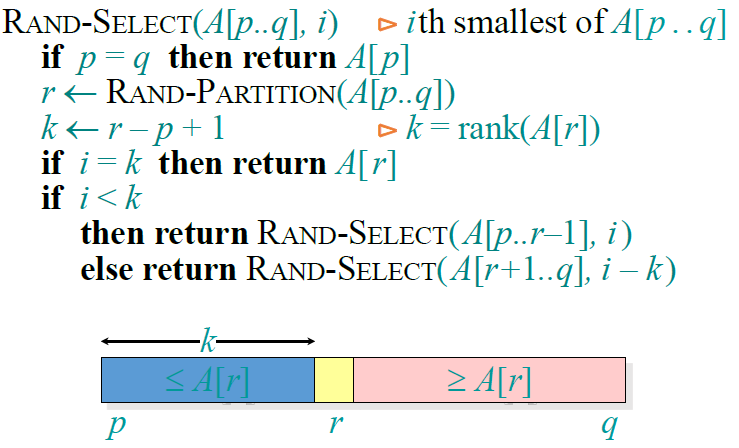
\includegraphics[width=\linewidth]{./images/randselect.png}

The idea is to randomly select a pivot then check the rank of the pivot, if the element we are looking for is int the left, recursively do it in the left sublist, if it is in the right, do so on the right

\subsubsection{Worst case linear time}
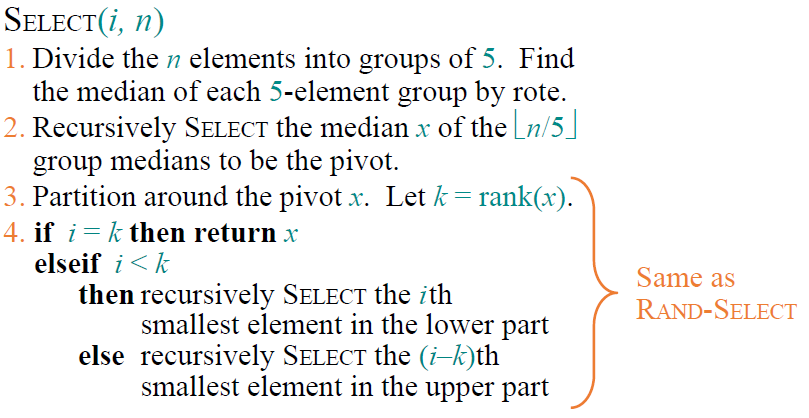
\includegraphics[width=\linewidth]{./images/worstcaseselect.png}
The idea is that we generate a good pivot each time, instead of randomly.
The median of the median of the groups has at least $3n/10$ elements greater or less than it.

\section{Week 7-Amortized Analysis}
\textbf{Amortized analysisis} a strategy for analyzing a sequence of operations to show that the average cost per operation is small, even though a single operation within the sequence might be expensive. Without the use of probability.

Consider the following case: We have a dynamic array initially of size 1. When we insert, if the list is full (overflow) we copy over to a new array with twice the size
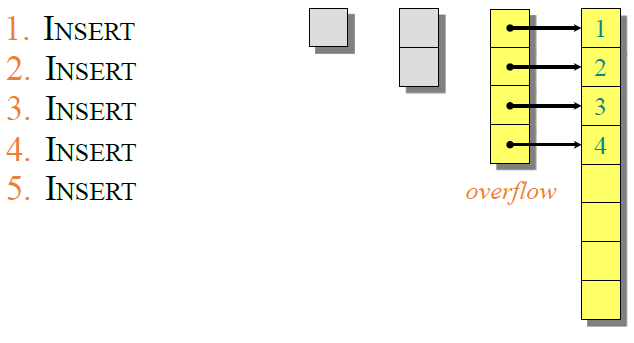
\includegraphics[width=\linewidth]{./images/dynamic.png}
Below are methods to perform amortized analysis
\subsection{Aggregate method}
The idea is that we use maths

Based on the problem above. Let $t(i)$ = the cost of the $i$th insertion
$$
=\begin{cases}
i & \text{if } $i-1$ is an exact power of 2\\
1 & \text{otherwise}
\end{cases}
$$
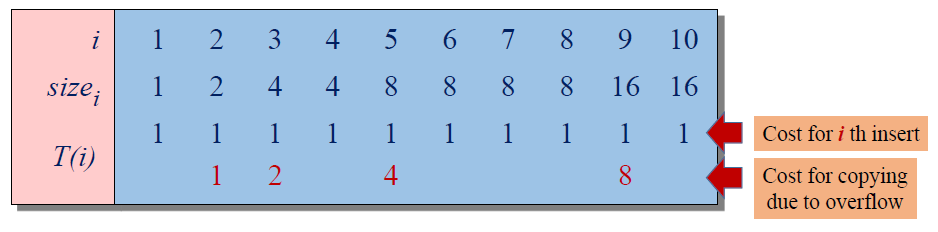
\includegraphics[width=\linewidth]{./images/aggregatetable.png}
Cost of $n$ insertions = $\sum_{i=1}^nt(i)$
\begin{align*}
&\leq n+ \Sigma_{j=0}^{\log (n-1)} 2^j\\
&\leq 3n
\end{align*}
Thus the average cost of each insertion in the dynamic array is $O(n)/n=O(1)$

\subsection{Accounting method}
The idea is to impose an extra charge on inexpensive operations and use it to pay for expensive operations later on. Excess money goes to the bank to be used for future operations. \textbf{Need to prove} that bank will never go negative.

Some observations in the problem above
\begin{itemize}
	\item at insertion $i$ overflow happens, thus next overflow at insertion $2i$
	\item between then there are $i$ insertions and we need to copy over $2i$ items.
\end{itemize}
Thus to find amortized cost
\begin{itemize}
	\item Each insertion is charged \$3
		\begin{itemize}
			\item \$1 is for the current insertion
			\item \$2 is stored to handle overflow
		\end{itemize}
	\item In the case of no overflow, insert for \$1 and store \$2
	\item In the case of overflow
		\begin{enumerate}
			\item Between this overflow and the previous overflow we have $i$
			\item So we have $\$2*i$ money in the bank,, use this to copy over, leaving $0$ in the bank
			\item The new item that caused the overflow is then inserted to the bigger array normally
		\end{enumerate}
\end{itemize}

\subsection{Potential method}
$\phi$: Potential function associated with the algorithm/data structure
$\phi(i)$: Potential at the end of the $i$th operation

Important conditions to be fulfilled by $\phi$
\begin{itemize}
	\item $\phi(0)=0$
	\item $\phi(i)\geq 0 \text{ for all } i$
\end{itemize}

Amortized cost of $i$th operation\\
=Actual cost of $i$th operation + $( \, \Delta \phi(i))\,$\\
=cost of $i$th operation + $( \,\phi(i)-\phi(i-1))\,$

\vspace{5mm} %5mm vertical space
Amortized cost of $n$ operations\\
=$\Sigma_i$Amortized cost of $i$th operation\\
=Actual cost of $n$ operations + $\phi(n)$\\
$\geq$ Actual cost of $n$ operations

Need to find a suitable Potential function $\phi$, so that for the costly operation $\Delta \phi_i$ is negative such that is nullifies or reduces the effect of the actual cost.\\
try to find what is decreasing in the expensive operation

\newpage
For the example above\\
$\phi(i)=2i-\text{size}(T)$
\begin{enumerate}
	\item $i$th insertion causes overflow. Actual cost= $i$. size=$i-1$ before new creation
		\begin{itemize}
			\item $\phi(i-1)=i-1$
			\item $phi(i)=2*i-2*(i-1)=2$
			\item $\Delta \phi_i=3-i$
		\end{itemize}
	\item $i$th insertion does not cause overflow. Actual cost = $1$. size = $l$
		\begin{itemize}
			\item $\phi(i-1)=2(i-1)-l$
			\item $\phi(i)=2i-l$
			\item $\Delta \phi_i=2$
		\end{itemize}
\end{enumerate}
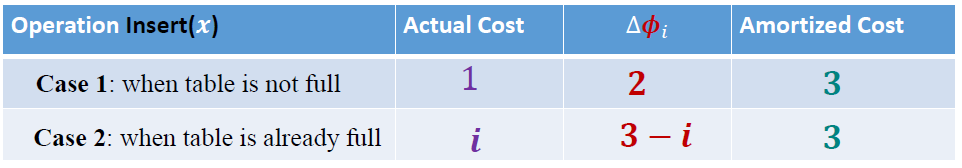
\includegraphics[width=\linewidth]{./images/potential.png}
 
\section{Week 8-Dynamic Programming}
Suppose we have a recursive solution\\
overall there are only a polynomial number of subproblems\\
And there is a huge overlap among the subproblems, the recursive algorithm takes exponential time because it solves the same problem many times)\\
So we compute the recursive solution iteratively in a bottom up manner, and memoize / remember past solutions to avoid wastage of computation 

\section{Week 9-Greedy Algorithm}
At each step of solving the algorithm, we need only solve one (greedy) sub problem each step.\\

Given a decision problem $P$\\
instance $A$ is of size $n$ of problem P\\
we perform a greedy step to reduce the problem to\\
instance $A'$ of size $<n$ of problem P

To prove that the greedy step is correct
\begin{enumerate}
	\item Try to establish a relation between OPT$(A)$ and OPT$(A')$
	\item Try to prove the relation formally by
		\begin{itemize}
			\item deriving a (not necessarily optimal) solution of $A$ from OPT$(A')$
			\item deriving a (not necessarily optimal) solution of $A'$ from OPT$(A)$
		\end{itemize}
	\item If you succeed, this algorithm is correct
\end{enumerate}
OPT denotes optimal algorithm to solve

\section{Week 10-Intractability}
To determine how hard a problem is, we use the idea of Reduction

A $\Rightarrow$ B

We take a general instance of the Problem $A$ transform it to a specific problem $B$
We can use some algorithm $M$ to solve $B$, then use solution to solve $A$

if $B$ is easy $\rightarrow$ $A$ is easy
if $A$ is hard $\rightarrow$ $B$ is hard


We focus on 
if $A$ is hard $\rightarrow$ $B$ is hard
$$A\leq_q B $$
make sure reduction is very fast, or else also no point
reduction must in polynomial time

\subsection{Optimization vs Decision}
Optimization:
\begin{itemize}
	\item give $^th$ min/max
	\item satisfy constraints
	\item ex: visit each city with min cost
\end{itemize}
	
Decision:
\begin{itemize}
	\item A problem instance, check is it solvable or not
	\item ex: can i visit every city within cost k
\end{itemize}

\subsection{Reductions between Decision Problems}
Given two decision problem $A$ and $B$, a polynomial time reduction from $A$ to $B$, denoted $A \leq_p B$, is a transformation from instance $\alpha$ of $A$ to instance $\beta$ of $B$ such that:
\begin{itemize}
\item Transformation must run in polynomial time in the size of $\alpha$. Word input encoding length
\item $\alpha$ is a YES-instance for $A$ if and only if $\beta$ is a YES-instance for $B$
	\begin{itemize}
		\item yes for B $\rightarrow$ yes for A
		\item yes for A $\rightarrow$ yes for B 
	\end{itemize}
\end{itemize}

\section{Week 11-NP completeness}
Complexity grouping:
\begin{itemize}
	\item P - (polynomial) - The set of decision problems which have efficient polytime algorithm
	\item NP - (Non-deterministic polynomial time) - The set of all decision problems which have efficient certifier
	\item NP-complete: A problem $X$ in NP class is NP-complete if\\for every $A\in \text{NP}, A\leq_pX$
	\item NP-Hard: A in NP $\leq_p$ B in NP hard.\\ If$X$ is not known to be in NP, then we just say $X$ is in NP-hard
\end{itemize}

How to show that a problem is NP-complete:
\begin{enumerate}
	\item Let $X$ be the problem we wish to prove is in NP-complete
	\item Show that $X\in \text{NP}$
	\item Pick a problem $A$ which is already known to be in NP-complete
	\item Show that $A\leq_pX$
\end{enumerate}
\section{Week 12-approximation}
Sometimes a problem is just too hard to solve, so we approximate the solution.\\
For an optimization problem, find a solution that is nearly optimal in cost

\subsection{Approximation Ratio}
Let $C^*$ be the optimal algorithm and $C$ be the cost of the solution given by an approximation algorithm.

An approximation algorithm $A$ has an approximation ratio $\rho(n)$ if:
\begin{itemize}
	\item for minimization problem $$\frac{C}{C^*}\leq \rho(n),\rho(n) \geq 1$$
	\item for maximization problem $$\frac{C}{C^*}\geq \rho(n),\rho(n) \leq 1$$
\end{itemize}
Here Cost refers to the maximization or minimization result C

\subsection{Analyzing Approximation Algorithms}
\begin{itemize}
	\item \textbf{Analyze a Heuristic}: A heuristic is a procedure that does not always produce the optimal answer, but we can show that it is not too bad. Compare heuristic with an optimal solution to find approximation ratio
	\item \textbf{Solve an Linear Programming relaxation}: Not Covered
\end{itemize}

\section{Problem Definitions and Algorithms}

\subsection{3-SAT}
is \textbf{NP-Complete}\\
\textbf{Definition}: SAT where each clause contains exactly 3 literals corresponding to different variables.\\
$$(\bar{x_1}\vee x_2 \vee x_3)\wedge (x_1 \vee \bar{x_2} \vee x_3)$$

\textbf{Optimization Version}:

\textbf{Decision Version}: Given a 3-SAT, does there exist a satisfying assignment

\subsection{Traveling Salesman Problem}
is \textbf{NP-Hard}\\
\textbf{Definition}: Given an undirected graph $G=(V,E)$, find a cycle that does through each vertex once and returns to the starting vertex.

\textbf{Optimization Version}: What is the shortest total distance of the cycle

\textbf{Decision Version}: Does there exist a cycle of total distance k

\subsection{Independent Set}
\textbf{Definition}: Given an undirected graph $G=(V,E)$, a subset $X\subseteq V$ is said to be an independent set if\\
For each $u,v\in X, (u,v)\notin E$\\
There is no edge connecting any two vertex in the independent set

\textbf{Optimization Version}: Compute Independent Set of largest size

\textbf{Decision Version}: Does there exist an independent set of size $>k$

\subsection{Vertex Cover}
is \textbf{NP-Complete}\\
\textbf{Definition}: Given a graph $G=(V,E)$, a vertex cover $V'$ is a subset of $V$ such that $\forall (u,v)\in E: u\in V' \vee v\in V'$\\
every edge has at least one end point in the vertex cover

\textbf{Optimization Version}: What is the smallest size of a vertex cover

\textbf{Decision Version}: Does there exist a vertex cover of size k

\subsection{Partition}
\textbf{Definition}: Given a set of positive integers set $S$, can the set be partitioned into two sets of equal total sum.

\subsection{Hamiltonian Cycle}
is \textbf{NP}\\
\textbf{Definition}: Given a graph $G$, Decide whether there is a simple cycle that visits each vertex exactly once.\\ 

\subsection{Max-Clique}
is \textbf{NP-Complete}\\
\textbf{Definition}:Given a graph $G=(V,E)$, does there exist a subset $V'$ of $V$, such that all vertices in $V'$ are adjacent to each other

\textbf{Optimization Version}: What is the largest max clique

\textbf{Decision Version}: Does there exist a max clique of size k

\subsection{Knapsack}
\textbf{Definition}: Given $n$ items described by non-negative integer pairs $(w_i,v_i)$, capacity $W$ and value $V$. $w_i$ denotes the weight of an item, $v_i$ denotes the value of the item.

\textbf{Optimization Version}: What is the maximum value a subset of item of total weight at most $W$ 

\textbf{Decision Version}: Is there a subset of item of total weight at most $W$ and total value at least $V$



\end{multicols*}
\end{document}
